\documentclass[11pt]{beamer}
\let\Tiny=\tiny

\usefonttheme[onlymath]{serif}

\usepackage{multicol}
\usepackage{amssymb,amsmath,amsthm,stmaryrd}
\usepackage{indentfirst}
\usepackage{latexsym}
\usepackage[utf8]{inputenc}
\usepackage{fancybox}
\usepackage{tikz}
\usepackage{tikz-qtree}
\usepackage{color}
\usepackage{colortbl}
\usepackage{eurosym}
\usepackage{listings}

\usetikzlibrary{trees,shapes,decorations}

\setbeamertemplate{navigation symbols}{}
\setbeamercovered{transparent}

\title[Language technologies and natural language processing]{A very short introduction to Language Technologies and Natural Language Processing}
\author{Jose F Quesada \& Jose Luis Pro}
\date{}

\mode<presentation>{\usetheme[]{Warsaw}}

\setbeamertemplate{footline}
    {
      \leavevmode
      \hbox{\begin{beamercolorbox}[wd=.5\paperwidth,ht=2.5ex,dp=1.125ex,leftskip=.3cm plus1fill,rightskip=.3cm]{author in head/foot}
        \usebeamerfont{author in head/foot}\insertshorttitle%
      \end{beamercolorbox}%
      \begin{beamercolorbox}[wd=.5\paperwidth,ht=2.5ex,dp=1.125ex,leftskip=.3cm,rightskip=.3cm plus1fil]{title in head/foot}
        \usebeamerfont{title in head/foot}
					\hfill\insertframenumber\,/\,\inserttotalframenumber
      \end{beamercolorbox}}
      \vskip0pt
    }

% TODO QUITAR AL FINAL
\hypersetup{pdfpagemode=UseNone}

\begin{document}

\begin{frame}
\titlepage
\end{frame}

\section{Preliminaries}
\subsection{Type of languages}

\begin{frame}
\setbeamercolor{block title}{use=structure,fg=white,bg=red!75!black}
\setbeamercolor{block body}{use=structure,fg=black,bg=red!10!white}
	\begin{block}{Language}
		\begin{center}
			Set of conventional spoken or written symbols used for commucation between entities.\par
			\pause
			So we can see a language as the linking between meaning (semantic side) and expression (syntantic side).
		\end{center}
	\end{block}
	\pause
	\vspace{15pt}
	Types of languages
	\begin{itemize}
		\item \textbf{Natural languages:} Used for the communication between human beings.
		\item \textbf{Formal languages:} Used by computers and in mathematical areas.
	\end{itemize}
\end{frame}

\begin{frame}
	\setbeamercolor{block title}{use=structure,fg=white,bg=red!75!black}
	\setbeamercolor{block body}{use=structure,fg=black,bg=red!10!white}
	\begin{block}{Differences between natural and formal languages:}
		\begin{enumerate}
			\pause
			\item Computers don't understand natural languages, (normal) humans don't understand computer languages.
			\item Formal languages shouldn't have ambiguities, but natural languages do have.
		\end{enumerate}
	\end{block} 
	\vspace{10pt}
	\pause 
	\textbf{Language Technologies} (LT's) are the set of technologies that aim to create software that has some kind of knowledge about natural languages. \par
	\vspace{10pt}
	\pause
	\textbf{Natural language processing} (NLP) is the scientific field concerned with the interactions between computers and human by means of natural languages.
\end{frame}

\subsection{Applications}

\begin{frame}
	\setbeamercolor{block title}{use=structure,fg=white,bg=blue!75!black}
	\setbeamercolor{block body}{use=structure,fg=black,bg=blue!10!white}
	\begin{block}{Applications of Language Technologies:}
		\begin{enumerate}
			\vspace{5pt}
			\item Machine Translation.
			\pause
			\item Question - Answering.
			\pause
			\item Automatic Text Classification.
			\pause
			\item Automatic Text Summarization.
			\pause
			\item Social Analytics.
			\pause
			\item Sentiment Analysis.
			\pause
			\item \textbf{Dialogue Systems.}
			\vspace{5pt}
		\end{enumerate}
	\end{block}
\end{frame}

\begin{frame}
	Dialogue Systems (written or spoken) are also known as:
	\begin{itemize}
		\item Conversational interfaces.
		\item Chatbots.
	\end{itemize}
	\vspace{20pt}
	\setbeamercolor{block title}{use=structure,fg=white,bg=blue!75!black}
	\setbeamercolor{block body}{use=structure,fg=black,bg=blue!10!white}
	\begin{block}{Applications of Dialogue Systems:}
		\begin{enumerate}
			\vspace{5pt}
			\pause
			\item Information providers.
			\pause
			\item Transactional agents.
			\pause
			\item Educational and learning tutoring.
			\vspace{5pt}
		\end{enumerate}
	\end{block}
\end{frame}
\subsection{Ambiguities}

\begin{frame}
	\setbeamercolor{block title}{use=structure,fg=white,bg=red!75!black}
	\setbeamercolor{block body}{use=structure,fg=black,bg=red!10!white}
	\begin{block}{Dialogue systems main issue}
		\begin{center}
		\vspace{10pt}
		The most difficult challenge in the design of conversational interfaces are related with the highly \\ambigous nature of spoken languages.
		\vspace{10pt}
		\end{center}
	\end{block}
	\setbeamercolor{block title}{use=structure,fg=white,bg=green!75!black}
	\setbeamercolor{block body}{use=structure,fg=black,bg=green!10!white}
	\pause	
	\begin{block}{Example}
		\begin{center}
		\vspace{10pt}
		\texttt{Peter come yesterday.}\par
		\texttt{Yesterday Peter come.}
		\vspace{10pt}
		\end{center}
	\end{block}
	\pause
	\begin{center}
		Two syntatic expressions $\Longleftrightarrow$ One semantic form
	\end{center}
\end{frame}

\begin{frame}
	\setbeamercolor{block title}{use=structure,fg=white,bg=green!75!black}
	\setbeamercolor{block body}{use=structure,fg=black,bg=green!10!white}
	\begin{block}{Example}
		\begin{center}
		\vspace{10pt}
		\texttt{Peter said John came yesterday.}
		\vspace{10pt}
		\end{center}
	\end{block}
	\vspace{10pt}
	\pause
	\begin{itemize}
		\item Was it yesterday when Peter said that?
		\item Was it yesterday when John came?
	\end{itemize}
	\vspace{10pt}
	\pause
	\begin{center}
		One syntatic expression $\Longleftrightarrow$ Two semantic forms
	\end{center}
\end{frame}

\begin{frame}
	Humans can deal with these ambiguities applying what is called ``psicolinguistic preferences'' and, of course, logic and common-sense reasoning:
	\vspace{10pt}
	\pause
	\setbeamercolor{block title}{use=structure,fg=white,bg=green!75!black}
	\setbeamercolor{block body}{use=structure,fg=black,bg=green!10!white}
	\begin{block}{Example}
		\begin{center}
		\vspace{10pt}
		\texttt{Peter said John will come yesterday.}
		\vspace{10pt}
		\end{center}
	\end{block}
	\vspace{10pt}
	\pause
	From the computer point of view this sentence is such ambigous like previous one but humans know that nobody \textsl{``will come yesterday''}.
\end{frame}

\subsection{Architecture}

\begin{frame}
\frametitle{Dialogue System architecture}
	\begin{center}
		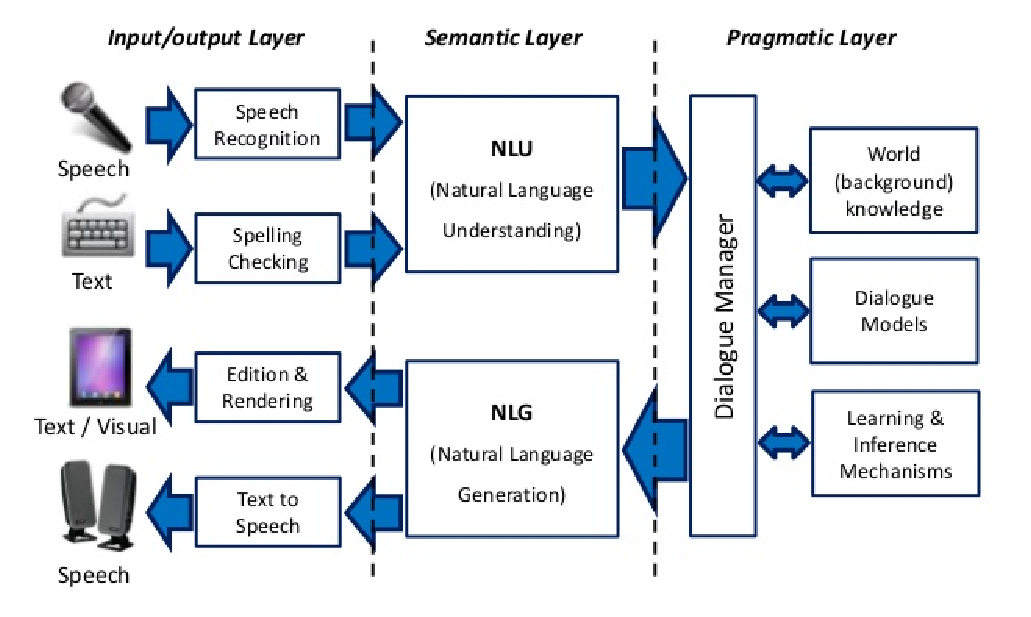
\includegraphics[width=1.00\textwidth]{ds.eps}
		\begin{tiny}
			Picture from Institute for Infocomm Research (Singapore)
		\end{tiny}
	\end{center}
\end{frame}

\section{Natural Language Understanding}
\subsection{Goal and meaning representation}

\begin{frame}
\frametitle{Natural Language Understanding (NLU)}
	\setbeamercolor{block title}{use=structure,fg=white,bg=red!75!black}
	\setbeamercolor{block body}{use=structure,fg=black,bg=red!10!white}
	\begin{block}{NLU main goal}
		\begin{center}
			\vspace{5pt}
			The goal of NLU stage is to transform an input string (let's say \textsl{user proference}) in an abstract representation of its meaning easier for computer programs to manipulate it, in order to execute some kind of reasoning.
			\vspace{5pt}
		\end{center}
	\end{block}
	\pause
	%\vspace{5pt}
	There is a wide variety of possible meaning representations.
	\begin{itemize}
		\item Topic maps.
		\item Concepts maps.
		\item Mind maps.
		\item Onthologies.
		\item \textbf{Feature structures.}
	\end{itemize}
\end{frame}

\begin{frame}
	\setbeamercolor{block title}{use=structure,fg=white,bg=green!75!black}
	\setbeamercolor{block body}{use=structure,fg=black,bg=green!10!white}
	\begin{block}{Example}
		\begin{center}
			\vspace{10pt}
				\texttt{John came yesterday} \small $\longrightarrow$ $\begin{bmatrix}
																				\textsc{Subject:}     & \texttt{John}\\ 
																				\textsc{Action:}      & \texttt{come}\\ 
																				\textsc{Tense:}     	& \texttt{past}\\ 
																				\textsc{Offsetdate:}  & \texttt{-1 day}\\ 
																			\end{bmatrix}$
			\vspace{10pt}
		\end{center}
	\end{block}
	\begin{block}{Example}
		\begin{center}
			\vspace{10pt}
				\texttt{John will talk in two days} \small $\longrightarrow$ $\begin{bmatrix}
																				\textsc{Subject:}     & \texttt{John}\\ 
																				\textsc{Action:}      & \texttt{talk}\\ 
																				\textsc{Tense:}     	& \texttt{future}\\ 
																				\textsc{Offsetdate:}  & \texttt{+2 day}\\ 
																			\end{bmatrix}$
			\vspace{10pt}
		\end{center}
	\end{block}
\end{frame}

\begin{frame}
	\setbeamercolor{block title}{use=structure,fg=white,bg=red!75!black}
	\setbeamercolor{block body}{use=structure,fg=black,bg=red!10!white}
	\begin{block}{Feature structures}
	\begin{itemize}
		\item A feature structure is a set of features.
		\item With no particular order between them.
		\item Every feature may have (but it's not required) an associated value.
		\item The value associated to every feature can be \textbf{atomic} or \textbf{complex}.
	\end{itemize}
	\end{block}
	\vspace{10pt}
	\pause
	\begin{center}
		\texttt{comes} \small $\longrightarrow$ 
				$\begin{bmatrix}
						\textsc{Action:}      & \texttt{come}\\ 
						\textsc{Tense:}     	& \texttt{present}\\ 
						\textsc{Agreement:}   & \begin{bmatrix}
																			\textsc{Number:} & \texttt{singular}\\ 
																			\textsc{Person:} & \texttt{3}\\ 
																		\end{bmatrix}
				\end{bmatrix}$
			\end{center}
\end{frame}

\subsection{Tokenizer, speller checker and POS tagging}

\begin{frame}
	\frametitle{NLU components}
	Trying to convert user proference to feature structures is not trivial. \par
	So we need to divide the process in some functional modules:
	\pause
	\vspace{10pt}
	\begin{itemize}
		\item Tokenization.
		\item Speller checker.
		\item Part Of Speech tagging (POS tagging).
		\item Parsing.
		\item Unifier.
	\end{itemize}
\end{frame}

\begin{frame}[fragile]
	\frametitle{Tokenization}
	\setbeamercolor{block title}{use=structure,fg=white,bg=red!75!black}
	\setbeamercolor{block body}{use=structure,fg=black,bg=red!10!white}
	\begin{block}{Goal}
		\begin{center}
			Convert a sequence of characters into a sequence of tokens.
		\end{center}
	\end{block}
	\pause
	We must take into account:
	\begin{itemize}
		\item Separators: \texttt{(\textvisiblespace -\char`_)}
		\item Punctuation marks: \texttt{(,.;:!?)}
		\item Special symbols: \texttt{(\$\euro\%º)}
		\item Numbers and its own separators: \texttt{(1234,.)}
		\item Alphanumeric codes: \texttt{(ES772024$\cdots$)}
	\end{itemize}
	\pause
	\setbeamercolor{block title}{use=structure,fg=white,bg=green!75!black}
	\setbeamercolor{block body}{use=structure,fg=black,bg=green!10!white}
	\begin{block}{Example}
	\begin{center}
		\begin{tabular}{ c c c c c c c c c c c c c c c c c }
			& tk1 & & tk2 & & tk3 & & tk4 & & tk5 & & tk6 \\
			$\cdot$ & The & $\cdot$ & dog & $\cdot$ & is & $\cdot$ & in & $\cdot$ & the & $\cdot$ & park & $\cdot$\\
			0 & & 1 & & 2 & & 3 & & 4 & & 5 & & 6
		\end{tabular}
	\end{center}
	\end{block}
\end{frame}

\begin{frame}
\frametitle{Speller checker (only in written dialogue systems)}
\begin{center}
	\Huge \texttt{London}
\end{center}
\begin{itemize}
	\item Insertion: \texttt{Loondon} 
	\item Deletion: \texttt{Lndon} 
	\item Substitution: \texttt{Lpndon} 
	\item Switching: \texttt{Lonodn} 
	\item Bad separators: \texttt{Lon don} 
\end{itemize}
\end{frame}

\begin{frame}
\frametitle{Part Of Speech tagging (POS tagging)}
	\setbeamercolor{block title}{use=structure,fg=white,bg=red!75!black}
	\setbeamercolor{block body}{use=structure,fg=black,bg=red!10!white}
	\begin{block}{Goal}
		\begin{center}
			To mark up lexical items with some lexical category depending on its definition and the context.
		\end{center}
	\end{block}
	\vspace{15pt}
	\pause
	In natural language we can have some common lexical categories:
	\begin{itemize}
		\item Determiners: \texttt{a, the} 
		\item Nouns: \texttt{London, dog} 
		\item Pronouns: \texttt{you, me} 
		\item Prepositions: \texttt{to, for} 
		\item Adjectives: \texttt{blue, long} 
	\end{itemize}
\end{frame}

\begin{frame}
\frametitle{POS tagging}
So in the lexicon definition we can classify lexical items into categories:\par
\begin{itemize}
	\item \texttt{("the", det)}
	\item \texttt{("dog", noun)}
	\item \texttt{("me", pronoun)}
	\item \texttt{("to", preposition)}
\end{itemize}
\vspace{5pt}
\pause
But in natural languages we can have several lexical categories corresponding to a single lexical item (especially in little inflectional ones, like in english): 
\begin{itemize}
	\item \texttt{("plans", noun)} $\longrightarrow$ plural of plan.
	\item \texttt{("plans", verb)} $\longrightarrow$ present of third person (singular) of verb to plan.
\end{itemize}
\end{frame}

\begin{frame}
\frametitle{POS tagging: Garden path problem}
	\setbeamercolor{block title}{use=structure,fg=white,bg=green!75!black}
	\setbeamercolor{block body}{use=structure,fg=black,bg=green!10!white}
	\begin{block}{Example}
		\begin{center}
		\begin{tabular}{ c c c c c c c c c c c c c c c c c }
			\underline{The} & \underline{\smash{government}} & \underline{\smash{plans}} & \underline{to} & \underline{raise} & \underline{taxes} & $\ldots$\\
			det & noun & \textbf{verb} & prep & verb & noun\\
		\end{tabular}
		\end{center}
	\end{block}
	\vspace{15pt}
	\pause
	\begin{block}{Example}
		\small
		\begin{center}
		\begin{tabular}{ c c c c c c c c c c c c c c c c c }
			\underline{The} & \underline{\smash{government}} & \underline{\smash{plans}} & \underline{to} & \underline{raise} & \underline{taxes} & \underline{were} & \underline{defeated}\\
			det & noun & \textbf{noun} & prep & verb & noun & verb & adj\\
		\end{tabular}
		\end{center}
	\end{block}
\end{frame}

\subsection{Grammars and parsing}

\begin{frame}
\frametitle{Formal grammars}
	\begin{itemize}
		\item Only study the purely syntactical aspects of language.
		\item \textbf{Alphabet:} Set of terminal symbols. $\{a,b\}$ 
		\item \textbf{Sentences:} Strings of symbols. $a,b,aa,ab,bb,ba,aaa,\cdots$ 
		\item \textbf{Language:} Set of sentences. $L = \{ab,aabb,aaabbb\}$
		\item \textbf{Formal grammar:} Set of formation rules used to define a language. $\{S\rightarrow a A,A\rightarrow b A,S\rightarrow\varepsilon\cdots\}$ Where $S, A$ are non-terminal symbols.
		\item Depending on the syntax of production rules, grammars can be classified (Noam Chomsky, 1956).
	\end{itemize}
\end{frame}

\begin{frame}
\frametitle{Chomsky grammar hierarchy}
	\small
	\begin{center}
		\begin{tabular}{ |c c c c| }
			\hline
			\textbf{Type} & \textbf{Grammar accepted} & \textbf{Rules} & \textbf{Observations}\\
			\hline
			Type 0 & Unrestricted grammar & $X \rightarrow Y$ & $X,Y \in (N\cup T)^*$\\
			\hline
			Type 1 & \begin{tabular}{@{}c@{}}Context-sensitive\\grammar\end{tabular} & $\alpha X \beta \rightarrow \alpha a \beta$ & \begin{tabular}{@{}c@{}}$X \in N$\\$\alpha,a,\beta \in (N\cup T)^
			*$\end{tabular}\\
			\hline
			\hline
			\rowcolor{yellow}Type 2 & Context-free grammar & $X \rightarrow a$ & \begin{tabular}{@{}c@{}}$X \in N$\\$a \in (N\cup T)^*$\end{tabular}\\
			\hline
			\hline
			Type 3 & Regular grammar & \begin{tabular}{@{}c@{}}$X \rightarrow a$\\$X \rightarrow aY$\end{tabular} & \begin{tabular}{@{}c@{}}$X,Y \in N$\\$X \in T$\end{tabular}\\
			\hline
		\end{tabular}
	\end{center}
	Where:
	\begin{itemize}
		\item $N$ is the set of non-terminal symbols.
		\item $T$ is the set of terminal symbols.
		\item $S^*$ is a string of elements in set $S$.
	\end{itemize}
\end{frame}

\begin{frame}
\frametitle{Easy context-free grammar example: $a^nb^m$}
	Consider:
	\begin{itemize}
		\item \textbf{Alphabet:} $\{a,b\}$ 
		\item \textbf{Language:} $L = \{a^nb^m\}\ n, m\geq 1$ (i.e. all strings with at least one ``a'' followed by at least one ``b'').
		\item \textbf{Grammar:} \begin{tabular}{l} $S \rightarrow a\ A\ b\ B$ \\ 
																							 $A \rightarrow \varepsilon$ \\
																							 $A \rightarrow a\ A$ \\
																							 $B \rightarrow \varepsilon$ \\
																							 $B \rightarrow b\ B$ \\
																						\end{tabular}
	\end{itemize}
	And let's see that a grammar defined with such production rules can be used to \textbf{generate} or either \textbf{recognize} the target language.
\end{frame}

\begin{frame}
\frametitle{Generating $a^nb^m$ sentences}
\begin{columns}
	\begin{column}{0.7\textwidth}
		\begin{center}
			\begin{tikzpicture}
			\tikzset{every tree node/.style={circle}}
			%\tikzset{level 1+/.style={level distance=2\baselineskip}}
			\tikzset{level 1+/.style={sibling distance=0.7\baselineskip}}
			%\tikzset{frontier/.style={distance from root=6\baselineskip}}
			\Tree [. S \edge[color=fg!0]; \node[color=fg!0]{a}; \edge[color=fg!0]; [.\node[color=fg!0]{A}; \edge[color=fg!0]; \node[color=fg!0]{a}; \edge[color=fg!0]; [.\node[color=fg!0]{A}; \edge[color=fg!0]; \node[color=fg!0]{a}; \edge[color=fg!0]; [.\node[color=fg!0]{A}; \edge[color=fg!0]; \node[color=fg!0]{$\varepsilon$}; ]]] \edge[color=fg!0]; \node[color=fg!0]{b}; \edge[color=fg!0]; [.\node[color=fg!0]{B}; \edge[color=fg!0]; \node[color=fg!0]{b}; \edge[color=fg!0]; [.\node[color=fg!0]{B}; \edge[color=fg!0]; \node[color=fg!0]{$\varepsilon$}; ]]]
			\end{tikzpicture}
		\end{center}
	\end{column}
	\begin{column}{0.3\textwidth}
		\begin{tabular}{l} $S \rightarrow a\ A\ b\ B$ \\ 
											 $A \rightarrow \varepsilon$ \\
											 $A \rightarrow a\ A$ \\
											 $B \rightarrow \varepsilon$ \\
											 $B \rightarrow b\ B$ \\
		\end{tabular}
	\end{column}
\end{columns}
\end{frame}

\begin{frame}[noframenumbering]
\frametitle{Generating $a^nb^m$ sentences}
\begin{columns}
	\begin{column}{0.7\textwidth}
		\begin{center}
			\begin{tikzpicture}
			\tikzset{every tree node/.style={circle}}
			%\tikzset{level 1+/.style={level distance=2\baselineskip}}
			\tikzset{level 1+/.style={sibling distance=0.7\baselineskip}}
			%\tikzset{frontier/.style={distance from root=6\baselineskip}}
			\Tree [. \node[fill=yellow]{S}; \edge[color=fg!0]; \node[color=fg!0]{a}; \edge[color=fg!0]; [.\node[color=fg!0]{A}; \edge[color=fg!0]; \node[color=fg!0]{a}; \edge[color=fg!0]; [.\node[color=fg!0]{A}; \edge[color=fg!0]; \node[color=fg!0]{a}; \edge[color=fg!0]; [.\node[color=fg!0]{A}; \edge[color=fg!0]; \node[color=fg!0]{$\varepsilon$}; ]]] \edge[color=fg!0]; \node[color=fg!0]{b}; \edge[color=fg!0]; [.\node[color=fg!0]{B}; \edge[color=fg!0]; \node[color=fg!0]{b}; \edge[color=fg!0]; [.\node[color=fg!0]{B}; \edge[color=fg!0]; \node[color=fg!0]{$\varepsilon$}; ]]]
			\end{tikzpicture}
		\end{center}
	\end{column}
	\begin{column}{0.3\textwidth}
		\begin{tabular}{l} \rowcolor{yellow}$S \rightarrow a\ A\ b\ B$ \\ 
											 $A \rightarrow \varepsilon$ \\
											 $A \rightarrow a\ A$ \\
											 $B \rightarrow \varepsilon$ \\
											 $B \rightarrow b\ B$ \\
		\end{tabular}
	\end{column}
\end{columns}
\end{frame}

\begin{frame}[noframenumbering]
\frametitle{Generating $a^nb^m$ sentences}
\begin{columns}
	\begin{column}{0.7\textwidth}
		\begin{center}
			\begin{tikzpicture}
			\tikzset{every tree node/.style={circle}}
			%\tikzset{level 1+/.style={level distance=2\baselineskip}}
			\tikzset{level 1+/.style={sibling distance=0.7\baselineskip}}
			%\tikzset{frontier/.style={distance from root=6\baselineskip}}
			\Tree [.S a [.A \edge[color=fg!0]; \node[color=fg!0]{a}; \edge[color=fg!0]; [.\node[color=fg!0]{A}; \edge[color=fg!0]; \node[color=fg!0]{a}; \edge[color=fg!0]; [.\node[color=fg!0]{A}; \edge[color=fg!0]; \node[color=fg!0]{$\varepsilon$}; ]]] b [.B \edge[color=fg!0]; \node[color=fg!0]{b}; \edge[color=fg!0]; [.\node[color=fg!0]{B}; \edge[color=fg!0]; \node[color=fg!0]{$\varepsilon$}; ]]]
			\end{tikzpicture}
		\end{center}
	\end{column}
	\begin{column}{0.3\textwidth}
		\begin{tabular}{l} $S \rightarrow a\ A\ b\ B$ \\ 
											 $A \rightarrow \varepsilon$ \\
											 $A \rightarrow a\ A$ \\
											 $B \rightarrow \varepsilon$ \\
											 $B \rightarrow b\ B$ \\
		\end{tabular}
	\end{column}
\end{columns}
\end{frame}

\begin{frame}[noframenumbering]
\frametitle{Generating $a^nb^m$ sentences}
\begin{columns}
	\begin{column}{0.7\textwidth}
		\begin{center}
			\begin{tikzpicture}
			\tikzset{every tree node/.style={circle}}
			%\tikzset{level 1+/.style={level distance=2\baselineskip}}
			\tikzset{level 1+/.style={sibling distance=0.7\baselineskip}}
			%\tikzset{frontier/.style={distance from root=6\baselineskip}}
			\Tree [.S a [.  \node[fill=yellow]{A}; \edge[color=fg!0]; \node[color=fg!0]{a}; \edge[color=fg!0]; [.\node[color=fg!0]{A}; \edge[color=fg!0]; \node[color=fg!0]{a}; \edge[color=fg!0]; [.\node[color=fg!0]{A}; \edge[color=fg!0]; \node[color=fg!0]{$\varepsilon$}; ]]] b [.B \edge[color=fg!0]; \node[color=fg!0]{b}; \edge[color=fg!0]; [.\node[color=fg!0]{B}; \edge[color=fg!0]; \node[color=fg!0]{$\varepsilon$}; ]]]
			\end{tikzpicture}
		\end{center}
	\end{column}
	\begin{column}{0.3\textwidth}
		\begin{tabular}{l} $S \rightarrow a\ A\ b\ B$ \\ 
											 $A \rightarrow \varepsilon$ \\
											 \rowcolor{yellow}$A \rightarrow a\ A$ \\
											 $B \rightarrow \varepsilon$ \\
											 $B \rightarrow b\ B$ \\
		\end{tabular}
	\end{column}
\end{columns}
\end{frame}

\begin{frame}[noframenumbering]
\frametitle{Generating $a^nb^m$ sentences}
\begin{columns}
	\begin{column}{0.7\textwidth}
		\begin{center}
			\begin{tikzpicture}
			\tikzset{every tree node/.style={circle}}
			%\tikzset{level 1+/.style={level distance=2\baselineskip}}
			\tikzset{level 1+/.style={sibling distance=0.7\baselineskip}}
			%\tikzset{frontier/.style={distance from root=6\baselineskip}}
			\Tree [.S a [.A a [.A \edge[color=fg!0]; \node[color=fg!0]{a}; \edge[color=fg!0]; [.\node[color=fg!0]{A}; \edge[color=fg!0]; \node[color=fg!0]{$\varepsilon$}; ]]] b [.B \edge[color=fg!0]; \node[color=fg!0]{b}; \edge[color=fg!0]; [.\node[color=fg!0]{B}; \edge[color=fg!0]; \node[color=fg!0]{$\varepsilon$}; ]]]
			\end{tikzpicture}
		\end{center}
	\end{column}
	\begin{column}{0.3\textwidth}
		\begin{tabular}{l} $S \rightarrow a\ A\ b\ B$ \\ 
											 $A \rightarrow \varepsilon$ \\
											 $A \rightarrow a\ A$ \\
											 $B \rightarrow \varepsilon$ \\
											 $B \rightarrow b\ B$ \\
		\end{tabular}
	\end{column}
\end{columns}
\end{frame}

\begin{frame}[noframenumbering]
\frametitle{Generating $a^nb^m$ sentences}
\begin{columns}
	\begin{column}{0.7\textwidth}
		\begin{center}
			\begin{tikzpicture}
			\tikzset{every tree node/.style={circle}}
			%\tikzset{level 1+/.style={level distance=2\baselineskip}}
			\tikzset{level 1+/.style={sibling distance=0.7\baselineskip}}
			%\tikzset{frontier/.style={distance from root=6\baselineskip}}
			\Tree [.S a [.A a [.\node[fill=yellow]{A}; \edge[color=fg!0]; \node[color=fg!0]{a}; \edge[color=fg!0]; [.\node[color=fg!0]{A}; \edge[color=fg!0]; \node[color=fg!0]{$\varepsilon$}; ]]] b [.B \edge[color=fg!0]; \node[color=fg!0]{b}; \edge[color=fg!0]; [.\node[color=fg!0]{B}; \edge[color=fg!0]; \node[color=fg!0]{$\varepsilon$}; ]]]
			\end{tikzpicture}
		\end{center}
	\end{column}
	\begin{column}{0.3\textwidth}
		\begin{tabular}{l} $S \rightarrow a\ A\ b\ B$ \\ 
											 $A \rightarrow \varepsilon$ \\
											 \rowcolor{yellow}$A \rightarrow a\ A$ \\
											 $B \rightarrow \varepsilon$ \\
											 $B \rightarrow b\ B$ \\
		\end{tabular}
	\end{column}
\end{columns}
\end{frame}

\begin{frame}[noframenumbering]
\frametitle{Generating $a^nb^m$ sentences}
\begin{columns}
	\begin{column}{0.7\textwidth}
		\begin{center}
			\begin{tikzpicture}
			\tikzset{every tree node/.style={circle}}
			%\tikzset{level 1+/.style={level distance=2\baselineskip}}
			\tikzset{level 1+/.style={sibling distance=0.7\baselineskip}}
			%\tikzset{frontier/.style={distance from root=6\baselineskip}}
			\Tree [.S a [.A a [.A a [.A \edge[color=fg!0]; \node[color=fg!0]{$\varepsilon$}; ]]] b [.B \edge[color=fg!0]; \node[color=fg!0]{b}; \edge[color=fg!0]; [.\node[color=fg!0]{B}; \edge[color=fg!0]; \node[color=fg!0]{$\varepsilon$}; ]]]
			\end{tikzpicture}
		\end{center}
	\end{column}
	\begin{column}{0.3\textwidth}
		\begin{tabular}{l} $S \rightarrow a\ A\ b\ B$ \\ 
											 $A \rightarrow \varepsilon$ \\
											 $A \rightarrow a\ A$ \\
											 $B \rightarrow \varepsilon$ \\
											 $B \rightarrow b\ B$ \\
		\end{tabular}
	\end{column}
\end{columns}
\end{frame}

\begin{frame}[noframenumbering]
\frametitle{Generating $a^nb^m$ sentences}
\begin{columns}
	\begin{column}{0.7\textwidth}
		\begin{center}
			\begin{tikzpicture}
			\tikzset{every tree node/.style={circle}}
			%\tikzset{level 1+/.style={level distance=2\baselineskip}}
			\tikzset{level 1+/.style={sibling distance=0.7\baselineskip}}
			%\tikzset{frontier/.style={distance from root=6\baselineskip}}
			\Tree [.S a [.A a [.A a [.\node[fill=yellow]{A}; \edge[color=fg!0]; \node[color=fg!0]{$\varepsilon$}; ]]] b [.B \edge[color=fg!0]; \node[color=fg!0]{b}; \edge[color=fg!0]; [.\node[color=fg!0]{B}; \edge[color=fg!0]; \node[color=fg!0]{$\varepsilon$}; ]]]
			\end{tikzpicture}
		\end{center}
	\end{column}
	\begin{column}{0.3\textwidth}
		\begin{tabular}{l} $S \rightarrow a\ A\ b\ B$ \\ 
											 \rowcolor{yellow}$A \rightarrow \varepsilon$ \\
											 $A \rightarrow a\ A$ \\
											 $B \rightarrow \varepsilon$ \\
											 $B \rightarrow b\ B$ \\
		\end{tabular}
	\end{column}
\end{columns}
\end{frame}

\begin{frame}[noframenumbering]
\frametitle{Generating $a^nb^m$ sentences}
\begin{columns}
	\begin{column}{0.7\textwidth}
		\begin{center}
			\begin{tikzpicture}
			\tikzset{every tree node/.style={circle}}
			%\tikzset{level 1+/.style={level distance=2\baselineskip}}
			\tikzset{level 1+/.style={sibling distance=0.7\baselineskip}}
			%\tikzset{frontier/.style={distance from root=6\baselineskip}}
			\Tree [.S a [.A a [.A a [.A $\varepsilon$ ]]] b [.B \edge[color=fg!0]; \node[color=fg!0]{b}; \edge[color=fg!0]; [.\node[color=fg!0]{B}; \edge[color=fg!0]; \node[color=fg!0]{$\varepsilon$}; ]]]
			\end{tikzpicture}
		\end{center}
	\end{column}
	\begin{column}{0.3\textwidth}
		\begin{tabular}{l} $S \rightarrow a\ A\ b\ B$ \\ 
											 $A \rightarrow \varepsilon$ \\
											 $A \rightarrow a\ A$ \\
											 $B \rightarrow \varepsilon$ \\
											 $B \rightarrow b\ B$ \\
		\end{tabular}
	\end{column}
\end{columns}
\end{frame}

\begin{frame}[noframenumbering]
\frametitle{Generating $a^nb^m$ sentences}
\begin{columns}
	\begin{column}{0.7\textwidth}
		\begin{center}
			\begin{tikzpicture}
			\tikzset{every tree node/.style={circle}}
			%\tikzset{level 1+/.style={level distance=2\baselineskip}}
			\tikzset{level 1+/.style={sibling distance=0.7\baselineskip}}
			%\tikzset{frontier/.style={distance from root=6\baselineskip}}
			\Tree [.S a [.A a [.A a [.A $\varepsilon$ ]]] b [.\node[fill=yellow]{B}; \edge[color=fg!0]; \node[color=fg!0]{b}; \edge[color=fg!0]; [.\node[color=fg!0]{B}; \edge[color=fg!0]; \node[color=fg!0]{$\varepsilon$}; ]]]
			\end{tikzpicture}
		\end{center}
	\end{column}
	\begin{column}{0.3\textwidth}
		\begin{tabular}{l} $S \rightarrow a\ A\ b\ B$ \\ 
											 $A \rightarrow \varepsilon$ \\
											 $A \rightarrow a\ A$ \\
											 $B \rightarrow \varepsilon$ \\
											 \rowcolor{yellow}$B \rightarrow b\ B$ \\
		\end{tabular}
	\end{column}
\end{columns}
\end{frame}

\begin{frame}[noframenumbering]
\frametitle{Generating $a^nb^m$ sentences}
\begin{columns}
	\begin{column}{0.7\textwidth}
		\begin{center}
			\begin{tikzpicture}
			\tikzset{every tree node/.style={circle}}
			%\tikzset{level 1+/.style={level distance=2\baselineskip}}
			\tikzset{level 1+/.style={sibling distance=0.7\baselineskip}}
			%\tikzset{frontier/.style={distance from root=6\baselineskip}}
			\Tree [.S a [.A a [.A a [.A $\varepsilon$ ]]] b [.B b [.B \edge[color=fg!0]; \node[color=fg!0]{$\varepsilon$}; ]]]
			\end{tikzpicture}
		\end{center}
	\end{column}
	\begin{column}{0.3\textwidth}
		\begin{tabular}{l} $S \rightarrow a\ A\ b\ B$ \\ 
											 $A \rightarrow \varepsilon$ \\
											 $A \rightarrow a\ A$ \\
											 $B \rightarrow \varepsilon$ \\
											 $B \rightarrow b\ B$ \\
		\end{tabular}
	\end{column}
\end{columns}
\end{frame}

\begin{frame}[noframenumbering]
\frametitle{Generating $a^nb^m$ sentences}
\begin{columns}
	\begin{column}{0.7\textwidth}
		\begin{center}
			\begin{tikzpicture}
			\tikzset{every tree node/.style={circle}}
			%\tikzset{level 1+/.style={level distance=2\baselineskip}}
			\tikzset{level 1+/.style={sibling distance=0.7\baselineskip}}
			%\tikzset{frontier/.style={distance from root=6\baselineskip}}
			\Tree [.S a [.A a [.A a [.A $\varepsilon$ ]]] b [.B b [.\node[fill=yellow]{B}; \edge[color=fg!0]; \node[color=fg!0]{$\varepsilon$}; ]]]
			\end{tikzpicture}
		\end{center}
	\end{column}
	\begin{column}{0.3\textwidth}
		\begin{tabular}{l} $S \rightarrow a\ A\ b\ B$ \\ 
											 $A \rightarrow \varepsilon$ \\
											 $A \rightarrow a\ A$ \\
											 \rowcolor{yellow}$B \rightarrow \varepsilon$ \\
											 $B \rightarrow b\ B$ \\
		\end{tabular}
	\end{column}
\end{columns}
\end{frame}

\begin{frame}[noframenumbering]
\frametitle{So we have generated $aaabb$ sentence!}
\begin{columns}
	\begin{column}{0.7\textwidth}
		\begin{center}
			\begin{tikzpicture}
			\tikzset{every tree node/.style={circle}}
			%\tikzset{level 1+/.style={level distance=2\baselineskip}}
			\tikzset{level 1+/.style={sibling distance=0.7\baselineskip}}
			%\tikzset{frontier/.style={distance from root=6\baselineskip}}
			\Tree [.S a [.A a [.A a [.A $\varepsilon$ ]]] b [.B b [.B $\varepsilon$ ]]]
			\end{tikzpicture}
		\end{center}
	\end{column}
	\begin{column}{0.3\textwidth}
		\begin{tabular}{l} $S \rightarrow a\ A\ b\ B$ \\ 
											 $A \rightarrow \varepsilon$ \\
											 $A \rightarrow a\ A$ \\
											 $B \rightarrow \varepsilon$ \\
											 $B \rightarrow b\ B$ \\
		\end{tabular}
	\end{column}
\end{columns}
\end{frame}

\begin{frame}
\frametitle{Recognizing $aaabb$ sentence}
\begin{columns}
	\begin{column}{0.7\textwidth}
		\begin{center}
			\begin{tikzpicture}
			\tikzset{every tree node/.style={circle}}
			%\tikzset{level 1+/.style={level distance=2\baselineskip}}
			\tikzset{level 1+/.style={sibling distance=0.7\baselineskip}}
			%\tikzset{frontier/.style={distance from root=6\baselineskip}}
			\Tree [. \node[color=fg!0]{S}; \edge[color=fg!0]; a \edge[color=fg!0]; [.\node[color=fg!0]{A}; \edge[color=fg!0]; a \edge[color=fg!0]; [.\node[color=fg!0]{A}; \edge[color=fg!0]; a \edge[color=fg!0]; [.\node[color=fg!0]{A}; \edge[color=fg!0]; \node[color=fg!0]{$\varepsilon$}; ]]] \edge[color=fg!0]; b \edge[color=fg!0]; [.\node[color=fg!0]{B}; \edge[color=fg!0]; b \edge[color=fg!0]; [.\node[color=fg!0]{B}; \edge[color=fg!0]; \node[color=fg!0]{$\varepsilon$}; ]]]
			\end{tikzpicture}
		\end{center}
	\end{column}
	\begin{column}{0.3\textwidth}
		\begin{tabular}{l} $S \rightarrow a\ A\ b\ B$ \\ 
											 $A \rightarrow \varepsilon$ \\
											 $A \rightarrow a\ A$ \\
											 $B \rightarrow \varepsilon$ \\
											 $B \rightarrow b\ B$ \\
		\end{tabular}
	\end{column}
\end{columns}
\end{frame}

\begin{frame}[noframenumbering]
\frametitle{Recognizing $aaabb$ sentence}
\begin{columns}
	\begin{column}{0.7\textwidth}
		\begin{center}
			\begin{tikzpicture}
			\tikzset{every tree node/.style={circle}}
			%\tikzset{level 1+/.style={level distance=2\baselineskip}}
			\tikzset{level 1+/.style={sibling distance=0.7\baselineskip}}
			%\tikzset{frontier/.style={distance from root=6\baselineskip}}
			\Tree [. \node[color=fg!0]{S}; \edge[color=fg!0]; a \edge[color=fg!0]; [.\node[color=fg!0]{A}; \edge[color=fg!0]; a \edge[color=fg!0]; [.\node[color=fg!0]{A}; \edge[color=fg!0]; a \edge[color=fg!0]; [.\node[color=fg!0]{A}; \edge[color=fg!0]; $\varepsilon$ ]]] \edge[color=fg!0]; b \edge[color=fg!0]; [.\node[color=fg!0]{B}; \edge[color=fg!0]; b \edge[color=fg!0]; [.\node[color=fg!0]{B}; \edge[color=fg!0]; $\varepsilon$ ]]]
			\end{tikzpicture}
		\end{center}
	\end{column}
	\begin{column}{0.3\textwidth}
		\begin{tabular}{l} $S \rightarrow a\ A\ b\ B$ \\ 
											 $A \rightarrow \varepsilon$ \\
											 $A \rightarrow a\ A$ \\
											 $B \rightarrow \varepsilon$ \\
											 $B \rightarrow b\ B$ \\
		\end{tabular}
	\end{column}
\end{columns}
\end{frame}

\begin{frame}[noframenumbering]
\frametitle{Recognizing $aaabb$ sentence}
\begin{columns}
	\begin{column}{0.7\textwidth}
		\begin{center}
			\begin{tikzpicture}
			\tikzset{every tree node/.style={circle}}
			%\tikzset{level 1+/.style={level distance=2\baselineskip}}
			\tikzset{level 1+/.style={sibling distance=0.7\baselineskip}}
			%\tikzset{frontier/.style={distance from root=6\baselineskip}}
			\Tree [. \node[color=fg!0]{S}; \edge[color=fg!0]; a \edge[color=fg!0]; [.\node[color=fg!0]{A}; \edge[color=fg!0]; a \edge[color=fg!0]; [.\node[color=fg!0]{A}; \edge[color=fg!0]; a \edge[color=fg!0]; [.\node[color=fg!0]{A}; \edge[color=fg!0]; \node[fill=yellow]{$\varepsilon$}; ]]] \edge[color=fg!0]; b \edge[color=fg!0]; [.\node[color=fg!0]{B}; \edge[color=fg!0]; b \edge[color=fg!0]; [.\node[color=fg!0]{B}; \edge[color=fg!0]; \node[fill=yellow]{$\varepsilon$}; ]]]
			\end{tikzpicture}
		\end{center}
	\end{column}
	\begin{column}{0.3\textwidth}
		\begin{tabular}{l} $S \rightarrow a\ A\ b\ B$ \\ 
											 \rowcolor{yellow}$A \rightarrow \varepsilon$ \\
											 $A \rightarrow a\ A$ \\
											 \rowcolor{yellow}$B \rightarrow \varepsilon$ \\
											 $B \rightarrow b\ B$ \\
		\end{tabular}
	\end{column}
\end{columns}
\end{frame}

\begin{frame}[noframenumbering]
\frametitle{Recognizing $aaabb$ sentence}
\begin{columns}
	\begin{column}{0.7\textwidth}
		\begin{center}
			\begin{tikzpicture}
			\tikzset{every tree node/.style={circle}}
			%\tikzset{level 1+/.style={level distance=2\baselineskip}}
			\tikzset{level 1+/.style={sibling distance=0.7\baselineskip}}
			%\tikzset{frontier/.style={distance from root=6\baselineskip}}
			\Tree [. \node[color=fg!0]{S}; \edge[color=fg!0]; a \edge[color=fg!0]; [.\node[color=fg!0]{A}; \edge[color=fg!0]; a \edge[color=fg!0]; [.\node[color=fg!0]{A}; \edge[color=fg!0]; a \edge[color=fg!0]; [.A $\varepsilon$ ]]] \edge[color=fg!0]; b \edge[color=fg!0]; [.\node[color=fg!0]{B}; \edge[color=fg!0]; b \edge[color=fg!0]; [.B $\varepsilon$ ]]]
			\end{tikzpicture}
		\end{center}
	\end{column}
	\begin{column}{0.3\textwidth}
		\begin{tabular}{l} $S \rightarrow a\ A\ b\ B$ \\ 
											 $A \rightarrow \varepsilon$ \\
											 $A \rightarrow a\ A$ \\
											 $B \rightarrow \varepsilon$ \\
											 $B \rightarrow b\ B$ \\
		\end{tabular}
	\end{column}
\end{columns}
\end{frame}

\begin{frame}[noframenumbering]
\frametitle{Recognizing $aaabb$ sentence}
\begin{columns}
	\begin{column}{0.7\textwidth}
		\begin{center}
			\begin{tikzpicture}
			\tikzset{every tree node/.style={circle}}
			%\tikzset{level 1+/.style={level distance=2\baselineskip}}
			\tikzset{level 1+/.style={sibling distance=0.7\baselineskip}}
			%\tikzset{frontier/.style={distance from root=6\baselineskip}}
			\Tree [. \node[color=fg!0]{S}; \edge[color=fg!0]; a \edge[color=fg!0]; [.\node[color=fg!0]{A}; \edge[color=fg!0]; a \edge[color=fg!0]; [.\node[color=fg!0]{A}; \edge[color=fg!0]; \node[fill=yellow]{a}; \edge[color=fg!0]; [.\node[fill=yellow]{A}; $\varepsilon$ ]]] \edge[color=fg!0]; b \edge[color=fg!0]; [.\node[color=fg!0]{B}; \edge[color=fg!0]; \node[fill=yellow]{b}; \edge[color=fg!0]; [.\node[fill=yellow]{B}; $\varepsilon$ ]]]
			\end{tikzpicture}
		\end{center}
	\end{column}
	\begin{column}{0.3\textwidth}
		\begin{tabular}{l} $S \rightarrow a\ A\ b\ B$ \\ 
											 $A \rightarrow \varepsilon$ \\
											 \rowcolor{yellow}$A \rightarrow a\ A$ \\
											 $B \rightarrow \varepsilon$ \\
											 \rowcolor{yellow}$B \rightarrow b\ B$ \\
		\end{tabular}
	\end{column}
\end{columns}
\end{frame}

\begin{frame}[noframenumbering]
\frametitle{Recognizing $aaabb$ sentence}
\begin{columns}
	\begin{column}{0.7\textwidth}
		\begin{center}
			\begin{tikzpicture}
			\tikzset{every tree node/.style={circle}}
			%\tikzset{level 1+/.style={level distance=2\baselineskip}}
			\tikzset{level 1+/.style={sibling distance=0.7\baselineskip}}
			%\tikzset{frontier/.style={distance from root=6\baselineskip}}
			\Tree [. \node[color=fg!0]{S}; \edge[color=fg!0]; a \edge[color=fg!0]; [.\node[color=fg!0]{A}; \edge[color=fg!0]; a \edge[color=fg!0]; [.A a [.A $\varepsilon$ ]]] \edge[color=fg!0]; b \edge[color=fg!0]; [.B b [.B $\varepsilon$ ]]]
			\end{tikzpicture}
		\end{center}
	\end{column}
	\begin{column}{0.3\textwidth}
		\begin{tabular}{l} $S \rightarrow a\ A\ b\ B$ \\ 
											 $A \rightarrow \varepsilon$ \\
											 $A \rightarrow a\ A$ \\
											 $B \rightarrow \varepsilon$ \\
											 $B \rightarrow b\ B$ \\
		\end{tabular}
	\end{column}
\end{columns}
\end{frame}

\begin{frame}[noframenumbering]
\frametitle{Recognizing $aaabb$ sentence}
\begin{columns}
	\begin{column}{0.7\textwidth}
		\begin{center}
			\begin{tikzpicture}
			\tikzset{every tree node/.style={circle}}
			%\tikzset{level 1+/.style={level distance=2\baselineskip}}
			\tikzset{level 1+/.style={sibling distance=0.7\baselineskip}}
			%\tikzset{frontier/.style={distance from root=6\baselineskip}}
			\Tree [. \node[color=fg!0]{S}; \edge[color=fg!0]; a \edge[color=fg!0]; [.\node[color=fg!0]{A}; \edge[color=fg!0]; \node[fill=yellow]{a}; \edge[color=fg!0]; [.\node[fill=yellow]{A}; a [.A $\varepsilon$ ]]] \edge[color=fg!0]; b \edge[color=fg!0]; [.B b [.B $\varepsilon$ ]]]
			\end{tikzpicture}
		\end{center}
	\end{column}
	\begin{column}{0.3\textwidth}
		\begin{tabular}{l} $S \rightarrow a\ A\ b\ B$ \\ 
											 $A \rightarrow \varepsilon$ \\
											 \rowcolor{yellow}$A \rightarrow a\ A$ \\
											 $B \rightarrow \varepsilon$ \\
											 $B \rightarrow b\ B$ \\
		\end{tabular}
	\end{column}
\end{columns}
\end{frame}

\begin{frame}[noframenumbering]
\frametitle{Recognizing $aaabb$ sentence}
\begin{columns}
	\begin{column}{0.7\textwidth}
		\begin{center}
			\begin{tikzpicture}
			\tikzset{every tree node/.style={circle}}
			%\tikzset{level 1+/.style={level distance=2\baselineskip}}
			\tikzset{level 1+/.style={sibling distance=0.7\baselineskip}}
			%\tikzset{frontier/.style={distance from root=6\baselineskip}}
			\Tree [. \node[color=fg!0]{S}; \edge[color=fg!0]; a \edge[color=fg!0]; [.A a [.A a [.A $\varepsilon$ ]]] \edge[color=fg!0]; b \edge[color=fg!0]; [.B b [.B $\varepsilon$ ]]]
			\end{tikzpicture}
		\end{center}
	\end{column}
	\begin{column}{0.3\textwidth}
		\begin{tabular}{l} $S \rightarrow a\ A\ b\ B$ \\ 
											 $A \rightarrow \varepsilon$ \\
											 $A \rightarrow a\ A$ \\
											 $B \rightarrow \varepsilon$ \\
											 $B \rightarrow b\ B$ \\
		\end{tabular}
	\end{column}
\end{columns}
\end{frame}

\begin{frame}[noframenumbering]
\frametitle{Recognizing $aaabb$ sentence}
\begin{columns}
	\begin{column}{0.7\textwidth}
		\begin{center}
			\begin{tikzpicture}
			\tikzset{every tree node/.style={circle}}
			%\tikzset{level 1+/.style={level distance=2\baselineskip}}
			\tikzset{level 1+/.style={sibling distance=0.7\baselineskip}}
			%\tikzset{frontier/.style={distance from root=6\baselineskip}}
			\Tree [. \node[color=fg!0]{S}; \edge[color=fg!0]; \node[fill=yellow]{a}; \edge[color=fg!0]; [.\node[fill=yellow]{A}; a [.A a [.A $\varepsilon$ ]]] \edge[color=fg!0]; \node[fill=yellow]{b}; \edge[color=fg!0]; [.\node[fill=yellow]{B}; b [.B $\varepsilon$ ]]]
			\end{tikzpicture}
		\end{center}
	\end{column}
	\begin{column}{0.3\textwidth}
		\begin{tabular}{l} \rowcolor{yellow}$S \rightarrow a\ A\ b\ B$ \\ 
											 $A \rightarrow \varepsilon$ \\
											 $A \rightarrow a\ A$ \\
											 $B \rightarrow \varepsilon$ \\
											 $B \rightarrow b\ B$ \\
		\end{tabular}
	\end{column}
\end{columns}
\end{frame}

\begin{frame}[noframenumbering]
\frametitle{We have recognized $aaabb$ sentence!}
\begin{columns}
	\begin{column}{0.7\textwidth}
		\begin{center}
			\begin{tikzpicture}
			\tikzset{every tree node/.style={circle}}
			%\tikzset{level 1+/.style={level distance=2\baselineskip}}
			\tikzset{level 1+/.style={sibling distance=0.7\baselineskip}}
			%\tikzset{frontier/.style={distance from root=6\baselineskip}}
			\Tree [.S a [.A a [.A a [.A $\varepsilon$ ]]] b [.B b [.B $\varepsilon$ ]]]
			\end{tikzpicture}
		\end{center}
	\end{column}
	\begin{column}{0.3\textwidth}
		\begin{tabular}{l} $S \rightarrow a\ A\ b\ B$ \\ 
											 $A \rightarrow \varepsilon$ \\
											 $A \rightarrow a\ A$ \\
											 $B \rightarrow \varepsilon$ \\
											 $B \rightarrow b\ B$ \\
		\end{tabular}
	\end{column}
\end{columns}
\end{frame}

\begin{frame}
	\setbeamercolor{block title}{use=structure,fg=white,bg=red!75!black}
	\setbeamercolor{block body}{use=structure,fg=black,bg=red!10!white}
	\begin{block}{Parsing}
		\begin{itemize}
			\item Is the process of analysing a sentence, according to the rules of a certain grammar, resulting in the creation of a ``parse tree''.
			\pause
			\item That parse tree includes syntactic relations between components in the sentence but may also contains semantic information (e.g. a feature structure).
		\end{itemize}
	\end{block}
	\pause
	\visible<3>{
	\begin{center}
		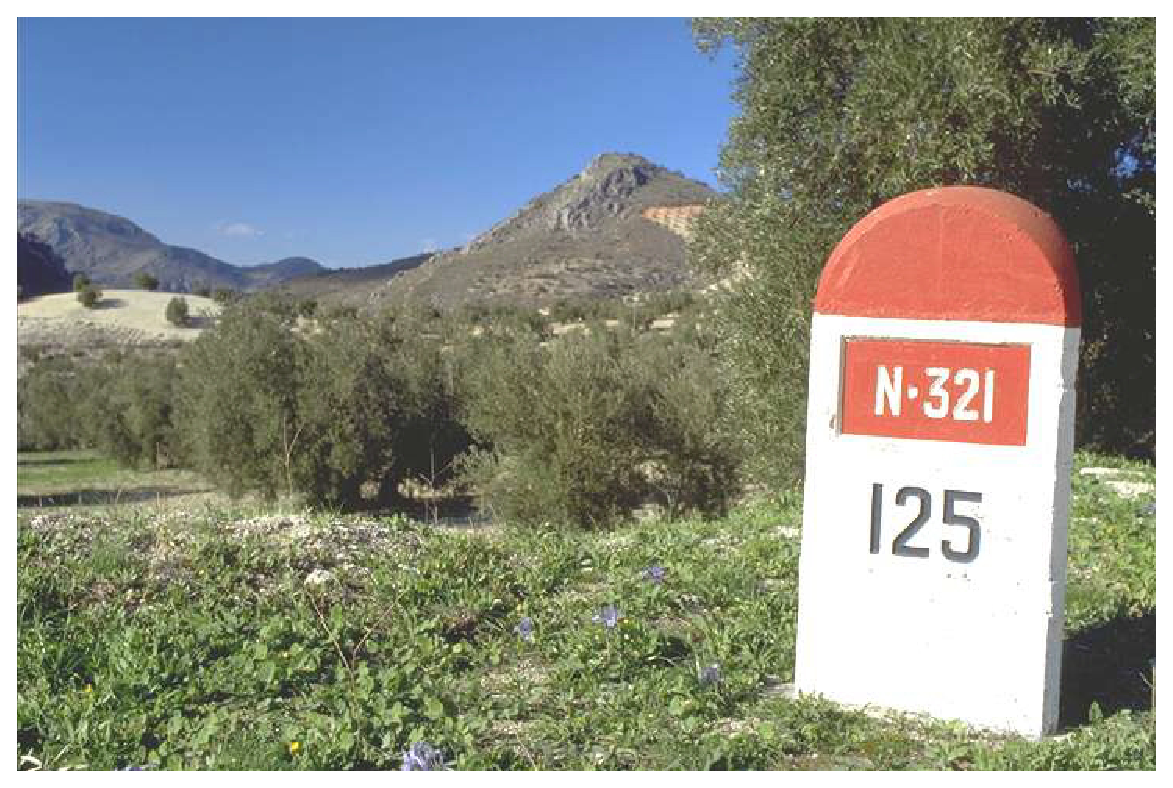
\includegraphics[width=0.54\textwidth]{milestone.eps}\\
		\begin{tiny}
			CC by Kat at the English language Wikipedia SA. 3.0
		\end{tiny}
	\end{center}}
\end{frame}

\begin{frame}
	\frametitle{Parsing applied to natural languages (english)}
	\begin{columns}
		\begin{column}{0.5\textwidth}
			Some typical lexical categories:
			\begin{itemize}
				\item \texttt{det}: Determiners.
				\item \texttt{noun}: Nouns.
				\item \texttt{verb}: Verbs.
				\item \texttt{prep}: Prepositions.
			\end{itemize}
			\pause
			\vspace{10pt}
			Some typical non-terminal symbols:
			\begin{itemize}
				\item \texttt{S}: Sentence.
				\item \texttt{NP}: Noun Phrase.
				\item \texttt{VP}: Verb Phrase.
				\item \texttt{PP}: Prepositional Phrase.
			\end{itemize}	
		\end{column}
		\pause
		\begin{column}{0.5\textwidth}
			Some typical production rules
			\begin{itemize}
				\item \texttt{S} $\rightarrow$ \texttt{NP} \texttt{VP}
				\item \texttt{NP} $\rightarrow$ \texttt{det} \texttt{noun}
				\item \texttt{VP} $\rightarrow$ \texttt{verb} 
				\item \texttt{VP} $\rightarrow$ \texttt{verb} \texttt{NP}
				\item \texttt{PP} $\rightarrow$ \texttt{prep} \texttt{NP}
				\item \texttt{NP} $\rightarrow$ \texttt{NP} \texttt{PP}
				\item \texttt{VP} $\rightarrow$ \texttt{VP} \texttt{PP}
			\end{itemize}
		\end{column}
	\end{columns}
\end{frame}

\begin{frame}
	\begin{columns}
	\begin{column}{0.7\textwidth}
		\begin{center}
			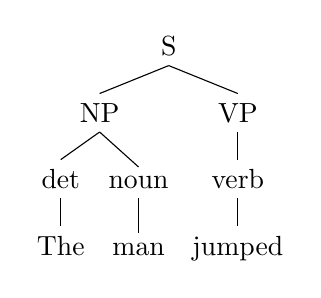
\begin{tikzpicture}
				\tikzset{every tree node/.style={align=center,anchor=base}}
				\tikzset{level 1+/.style={level distance=2\baselineskip}}
				\tikzset{frontier/.style={distance from root=6\baselineskip}}
				\Tree [.S [.NP [.det The ] [.noun man ] ] [.VP [.verb jumped ]]]
			\end{tikzpicture}
		\end{center}
	\end{column}
	\begin{column}{0.3\textwidth}
		\begin{tabular}{l} 	\rowcolor{yellow}\texttt{S} $\rightarrow$ \texttt{NP} \texttt{VP} \\
												\rowcolor{yellow}\texttt{NP} $\rightarrow$ \texttt{det} \texttt{noun} \\
												\rowcolor{yellow}\texttt{VP} $\rightarrow$ \texttt{verb}  \\
												\texttt{VP} $\rightarrow$ \texttt{verb} \texttt{NP} \\
												\texttt{PP} $\rightarrow$ \texttt{prep} \texttt{NP} \\
												\texttt{NP} $\rightarrow$ \texttt{NP} \texttt{PP} \\
												\texttt{VP} $\rightarrow$ \texttt{VP} \texttt{PP} \\
		\end{tabular}
	\end{column}
	\end{columns}
\end{frame}

\begin{frame}
	\begin{columns}
	\begin{column}{0.7\textwidth}
		\begin{center}
			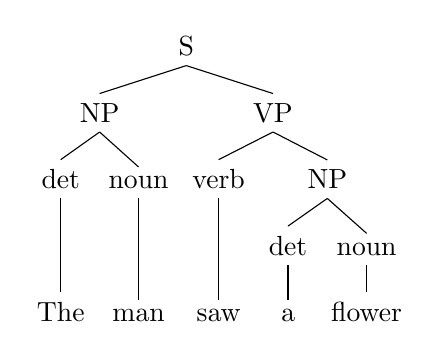
\begin{tikzpicture}
				\tikzset{every tree node/.style={align=center,anchor=base}}
				\tikzset{level 1+/.style={level distance=2\baselineskip}}
				\tikzset{frontier/.style={distance from root=8\baselineskip}}
				\Tree [.S [.NP [.det The ] [.noun man ] ] [.VP [.verb saw ] [.NP [.det a ] [.noun flower ]]]]
			\end{tikzpicture}
		\end{center}
	\end{column}
	\begin{column}{0.3\textwidth}
		\begin{tabular}{l} 	\rowcolor{yellow}\texttt{S} $\rightarrow$ \texttt{NP} \texttt{VP} \\
												\rowcolor{yellow}\texttt{NP} $\rightarrow$ \texttt{det} \texttt{noun} \\
												\texttt{VP} $\rightarrow$ \texttt{verb}  \\
												\rowcolor{yellow}\texttt{VP} $\rightarrow$ \texttt{verb} \texttt{NP} \\
												\texttt{PP} $\rightarrow$ \texttt{prep} \texttt{NP} \\
												\texttt{NP} $\rightarrow$ \texttt{NP} \texttt{PP} \\
												\texttt{VP} $\rightarrow$ \texttt{VP} \texttt{PP} \\
		\end{tabular}
	\end{column}
	\end{columns}
\end{frame}

\begin{frame}
	\begin{columns}
	\begin{column}{0.7\textwidth}
		\begin{center}
			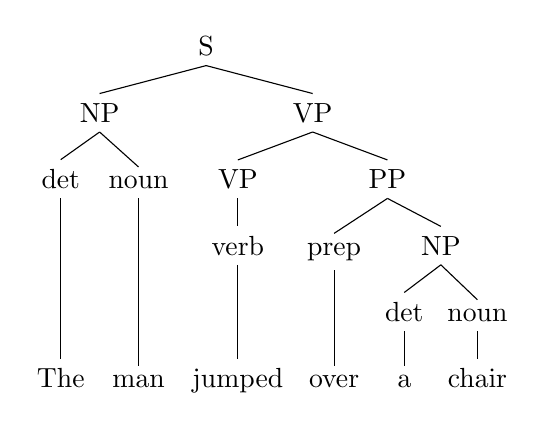
\begin{tikzpicture}
				\tikzset{every tree node/.style={align=center,anchor=base}}
				\tikzset{level 1+/.style={level distance=2\baselineskip}}
				\tikzset{frontier/.style={distance from root=10\baselineskip}}
				\Tree [.S [.NP [.det The ] [.noun man ] ] [.VP [.VP [.verb jumped ] ] [.PP [.prep over ] [.NP [.det a ] [.noun chair ] ]]]]
			\end{tikzpicture}
		\end{center}
	\end{column}
	\begin{column}{0.3\textwidth}
		\begin{tabular}{l} 	\rowcolor{yellow}\texttt{S} $\rightarrow$ \texttt{NP} \texttt{VP} \\
												\rowcolor{yellow}\texttt{NP} $\rightarrow$ \texttt{det} \texttt{noun} \\
												\rowcolor{yellow}\texttt{VP} $\rightarrow$ \texttt{verb}  \\
												\texttt{VP} $\rightarrow$ \texttt{verb} \texttt{NP} \\
												\rowcolor{yellow}\texttt{PP} $\rightarrow$ \texttt{prep} \texttt{NP} \\
												\texttt{NP} $\rightarrow$ \texttt{NP} \texttt{PP} \\
												\rowcolor{yellow}\texttt{VP} $\rightarrow$ \texttt{VP} \texttt{PP} \\
		\end{tabular}
	\end{column}
	\end{columns}
\end{frame}

\begin{frame}
	\begin{columns}
	\begin{column}{0.7\textwidth}
		\begin{center}
			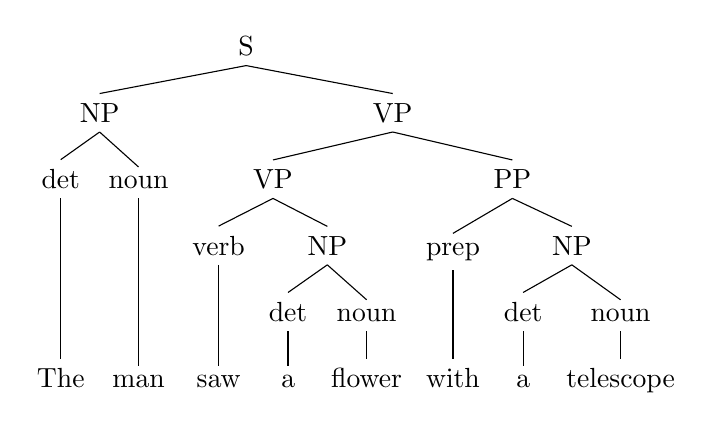
\begin{tikzpicture}
				\tikzset{every tree node/.style={align=center,anchor=base}}
				\tikzset{level 1+/.style={level distance=2\baselineskip}}
				\tikzset{frontier/.style={distance from root=10\baselineskip}}
				\Tree [.S [.NP [.det The ] [.noun man ] ] [.VP [.VP [.verb saw ] [.NP [.det a ] [.noun flower ] ] ] [.PP [.prep with ] [.NP [.det a ] [.noun telescope ] ]]]]
			\end{tikzpicture}
		\end{center}
	\end{column}
	\begin{column}{0.3\textwidth}
		\begin{tabular}{l} 	\rowcolor{yellow}\texttt{S} $\rightarrow$ \texttt{NP} \texttt{VP} \\
												\rowcolor{yellow}\texttt{NP} $\rightarrow$ \texttt{det} \texttt{noun} \\
												\texttt{VP} $\rightarrow$ \texttt{verb}  \\
												\rowcolor{yellow}\texttt{VP} $\rightarrow$ \texttt{verb} \texttt{NP} \\
												\rowcolor{yellow}\texttt{PP} $\rightarrow$ \texttt{prep} \texttt{NP} \\
												\texttt{NP} $\rightarrow$ \texttt{NP} \texttt{PP} \\
												\rowcolor{yellow}\texttt{VP} $\rightarrow$ \texttt{VP} \texttt{PP} \\
		\end{tabular}
	\end{column}
	\end{columns}
\end{frame}

\begin{frame}[noframenumbering]
	\begin{columns}
	\begin{column}{0.7\textwidth}
		\begin{center}
			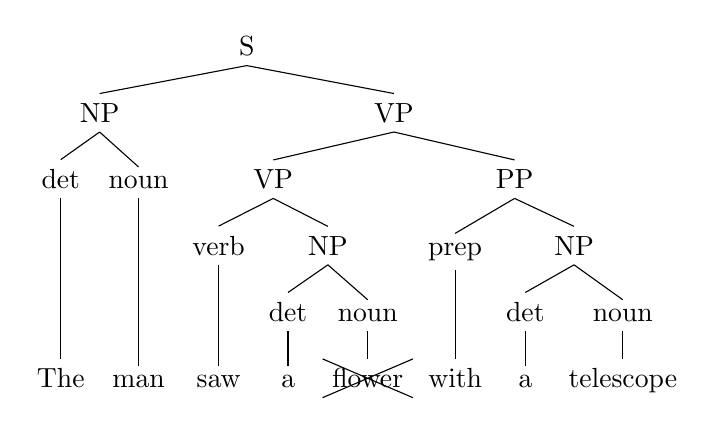
\begin{tikzpicture}
				\tikzset{every tree node/.style={align=center,anchor=base}}
				\tikzset{level 1+/.style={level distance=2\baselineskip}}
				\tikzset{frontier/.style={distance from root=10\baselineskip}}
				\Tree [.S [.NP [.det The ] [.noun man ] ] [.VP [.VP [.verb saw ] [.NP [.det a ] [.noun \node[draw,cross out]{flower}; ] ] ] [.PP [.prep with ] [.NP [.det a ] [.noun telescope ] ]]]]
			\end{tikzpicture}
		\end{center}
	\end{column}
	\begin{column}{0.3\textwidth}
		\begin{tabular}{l} 	\rowcolor{yellow}\texttt{S} $\rightarrow$ \texttt{NP} \texttt{VP} \\
												\rowcolor{yellow}\texttt{NP} $\rightarrow$ \texttt{det} \texttt{noun} \\
												\texttt{VP} $\rightarrow$ \texttt{verb}  \\
												\rowcolor{yellow}\texttt{VP} $\rightarrow$ \texttt{verb} \texttt{NP} \\
												\rowcolor{yellow}\texttt{PP} $\rightarrow$ \texttt{prep} \texttt{NP} \\
												\texttt{NP} $\rightarrow$ \texttt{NP} \texttt{PP} \\
												\rowcolor{yellow}\texttt{VP} $\rightarrow$ \texttt{VP} \texttt{PP} \\
		\end{tabular}
	\end{column}
	\end{columns}
\end{frame}

\begin{frame}[noframenumbering]
	\begin{columns}
	\begin{column}{0.7\textwidth}
		\begin{center}
			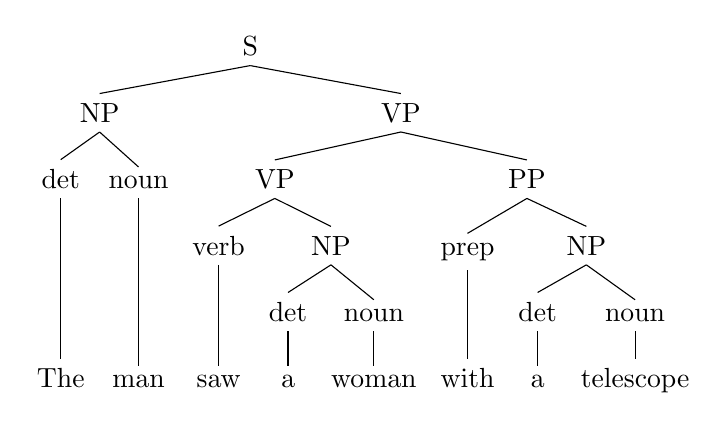
\begin{tikzpicture}
				\tikzset{every tree node/.style={align=center,anchor=base}}
				\tikzset{level 1+/.style={level distance=2\baselineskip}}
				\tikzset{frontier/.style={distance from root=10\baselineskip}}
				\Tree [.S [.NP [.det The ] [.noun man ] ] [.VP [.VP [.verb saw ] [.NP [.det a ] [.noun woman ] ] ] [.PP [.prep with ] [.NP [.det a ] [.noun telescope ] ]]]]
			\end{tikzpicture}
		\end{center}
	\end{column}
	\begin{column}{0.3\textwidth}
		\begin{tabular}{l} 	\rowcolor{yellow}\texttt{S} $\rightarrow$ \texttt{NP} \texttt{VP} \\
												\rowcolor{yellow}\texttt{NP} $\rightarrow$ \texttt{det} \texttt{noun} \\
												\texttt{VP} $\rightarrow$ \texttt{verb}  \\
												\rowcolor{yellow}\texttt{VP} $\rightarrow$ \texttt{verb} \texttt{NP} \\
												\rowcolor{yellow}\texttt{PP} $\rightarrow$ \texttt{prep} \texttt{NP} \\
												\texttt{NP} $\rightarrow$ \texttt{NP} \texttt{PP} \\
												\rowcolor{yellow}\texttt{VP} $\rightarrow$ \texttt{VP} \texttt{PP} \\
		\end{tabular}
	\end{column}
	\end{columns}
\end{frame}

\begin{frame}
	\begin{columns}
	\begin{column}{0.7\textwidth}
		\begin{center}
			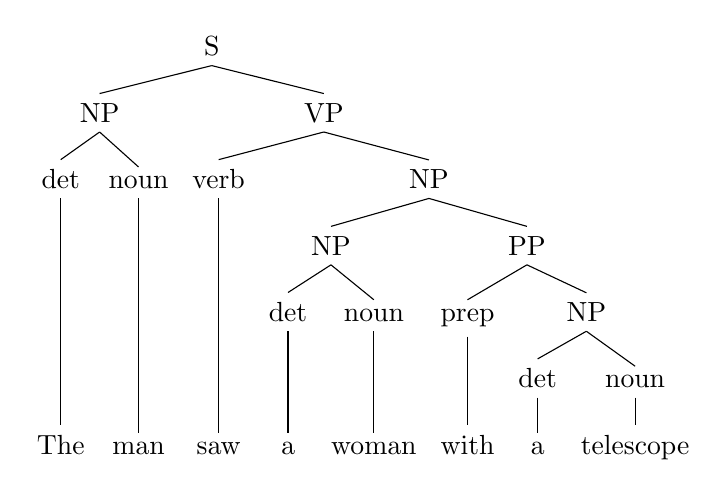
\begin{tikzpicture}
				\tikzset{every tree node/.style={align=center,anchor=base}}
				\tikzset{level 1+/.style={level distance=2\baselineskip}}
				\tikzset{frontier/.style={distance from root=12\baselineskip}}
				\Tree [.S [.NP [.det The ] [.noun man ] ] [.VP [.verb saw ] [.NP [.NP [.det a ] [.noun woman ] ] [.PP [.prep with ] [.NP [.det a ] [.noun telescope ] ] ] ] ] ] ]
			\end{tikzpicture}
		\end{center}
	\end{column}
	\begin{column}{0.3\textwidth}
		\begin{tabular}{l} 	\rowcolor{yellow}\texttt{S} $\rightarrow$ \texttt{NP} \texttt{VP} \\
												\rowcolor{yellow}\texttt{NP} $\rightarrow$ \texttt{det} \texttt{noun} \\
												\texttt{VP} $\rightarrow$ \texttt{verb}  \\
												\rowcolor{yellow}\texttt{VP} $\rightarrow$ \texttt{verb} \texttt{NP} \\
												\rowcolor{yellow}\texttt{PP} $\rightarrow$ \texttt{prep} \texttt{NP} \\
												\rowcolor{yellow}\texttt{NP} $\rightarrow$ \texttt{NP} \texttt{PP} \\
												\texttt{VP} $\rightarrow$ \texttt{VP} \texttt{PP} \\
		\end{tabular}
	\end{column}
	\end{columns}
\end{frame}

\begin{frame}
	\setbeamercolor{block title}{use=structure,fg=white,bg=red!75!black}
	\setbeamercolor{block body}{use=structure,fg=black,bg=red!10!white}
	\begin{block}{Conclusions}
		\begin{itemize}
			\item With so little production rules we have ambiguities.
			\pause
			\item In practice, creating a general grammar results in too much ambiguities and poor performance.
			\pause
			\item \textbf{Solution:} Create simple grammars for simple parameter extraction.
		\end{itemize}
	\end{block}
	\pause
	\visible<4>{
	\begin{center}
		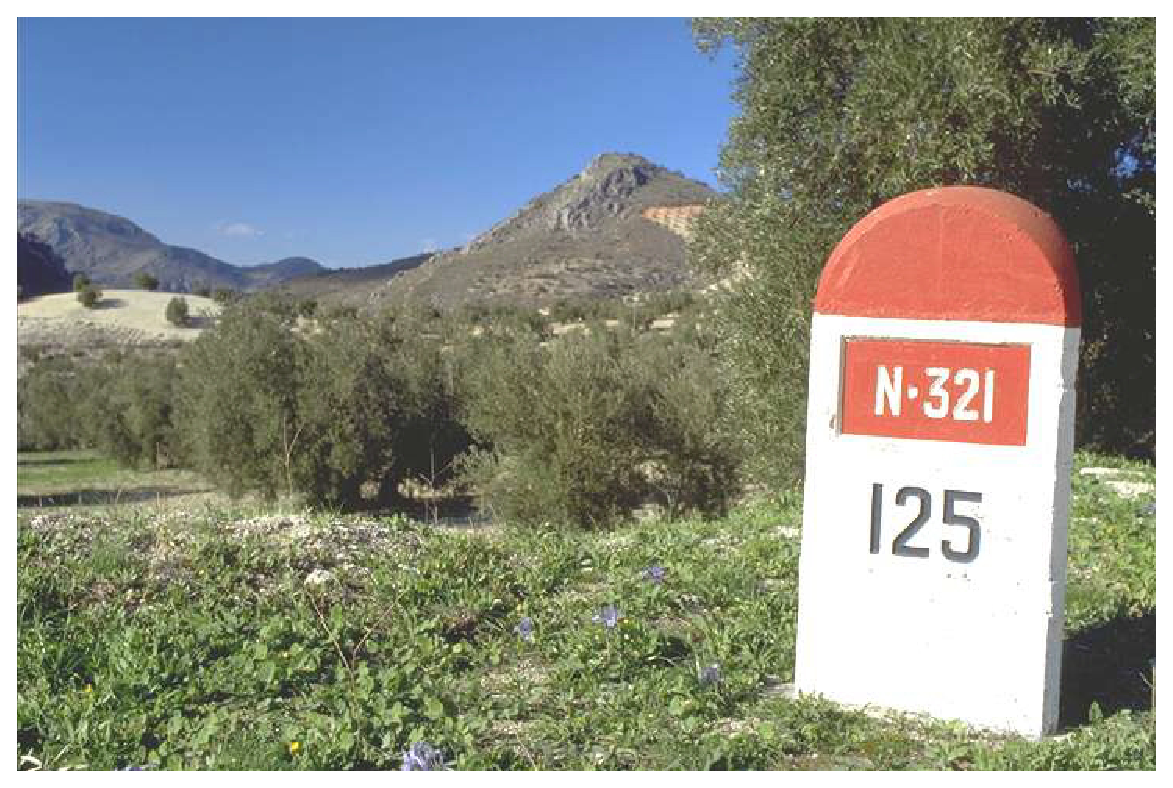
\includegraphics[width=0.5\textwidth]{milestone.eps}\\
		\begin{tiny}
			CC by Kat at the English language Wikipedia SA. 3.0
		\end{tiny}
	\end{center}}
\end{frame}

\subsection{Unifier}

\begin{frame}
\end{frame}

\section{Dialogue Manager}

\begin{frame}
\end{frame}

\section{Natural Language Generation}

\begin{frame}
\end{frame}

\end{document}
